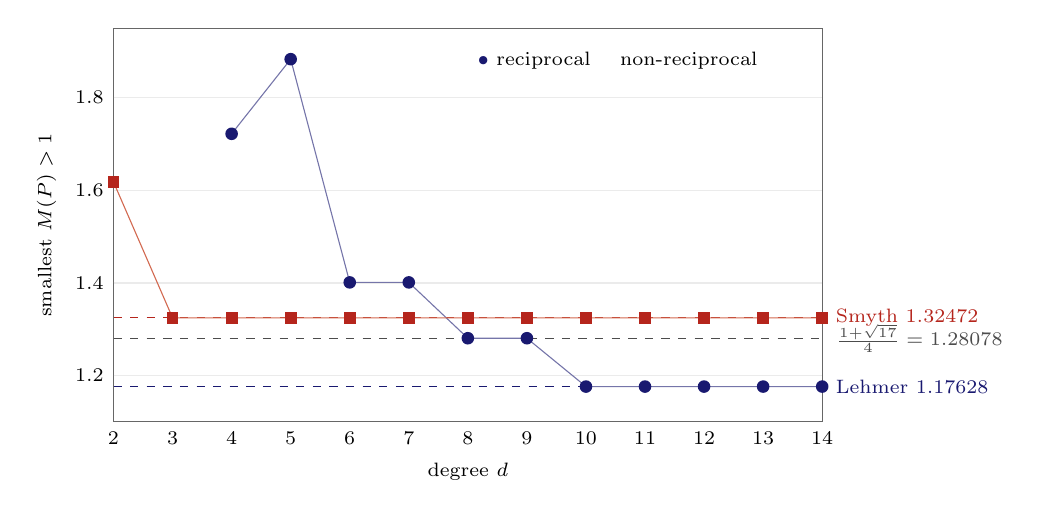
\begin{tikzpicture}[font=\scriptsize]
\draw[black!60] (0,0) rectangle (9.000,5.000);
\node[below] at (0.000,0) {$2$};
\node[below] at (0.750,0) {$3$};
\node[below] at (1.500,0) {$4$};
\node[below] at (2.250,0) {$5$};
\node[below] at (3.000,0) {$6$};
\node[below] at (3.750,0) {$7$};
\node[below] at (4.500,0) {$8$};
\node[below] at (5.250,0) {$9$};
\node[below] at (6.000,0) {$10$};
\node[below] at (6.750,0) {$11$};
\node[below] at (7.500,0) {$12$};
\node[below] at (8.250,0) {$13$};
\node[below] at (9.000,0) {$14$};
\draw[black!8] (0,0.588) -- (9.000,0.588); \node[left] at (0,0.588) {$1.2$};
\draw[black!8] (0,1.765) -- (9.000,1.765); \node[left] at (0,1.765) {$1.4$};
\draw[black!8] (0,2.941) -- (9.000,2.941); \node[left] at (0,2.941) {$1.6$};
\draw[black!8] (0,4.118) -- (9.000,4.118); \node[left] at (0,4.118) {$1.8$};
\draw[MidnightBlue,dashed] (0,0.449) -- (9.000,0.449); \node[right,MidnightBlue] at (9.050,0.449) {Lehmer $1.17628$};
\draw[black!70,dashed] (0,1.063) -- (9.000,1.063); \node[right,black!70] at (9.050,1.063) {$\frac{1+\sqrt{17}}4=1.28078$};
\draw[BrickRed,dashed] (0,1.322) -- (9.000,1.322); \node[right,BrickRed] at (9.050,1.322) {Smyth $1.32472$};
\draw[MidnightBlue!60] (1.500,3.659) -- (2.250,4.607) -- (3.000,1.772) -- (3.750,1.772) -- (4.500,1.063) -- (5.250,1.063) -- (6.000,0.449) -- (6.750,0.449) -- (7.500,0.449) -- (8.250,0.449) -- (9.000,0.449);
\fill[MidnightBlue] (1.500,3.659) circle (0.08);
\fill[MidnightBlue] (2.250,4.607) circle (0.08);
\fill[MidnightBlue] (3.000,1.772) circle (0.08);
\fill[MidnightBlue] (3.750,1.772) circle (0.08);
\fill[MidnightBlue] (4.500,1.063) circle (0.08);
\fill[MidnightBlue] (5.250,1.063) circle (0.08);
\fill[MidnightBlue] (6.000,0.449) circle (0.08);
\fill[MidnightBlue] (6.750,0.449) circle (0.08);
\fill[MidnightBlue] (7.500,0.449) circle (0.08);
\fill[MidnightBlue] (8.250,0.449) circle (0.08);
\fill[MidnightBlue] (9.000,0.449) circle (0.08);
\draw[BrickRed!60] (0.000,3.047) -- (0.750,1.322) -- (1.500,1.322) -- (2.250,1.322) -- (3.000,1.322) -- (3.750,1.322) -- (4.500,1.322) -- (5.250,1.322) -- (6.000,1.322) -- (6.750,1.322) -- (7.500,1.322) -- (8.250,1.322) -- (9.000,1.322);
\fill[BrickRed] (0.000,3.047) +(-0.075,-0.075) rectangle +(0.075,0.075);
\fill[BrickRed] (0.750,1.322) +(-0.075,-0.075) rectangle +(0.075,0.075);
\fill[BrickRed] (1.500,1.322) +(-0.075,-0.075) rectangle +(0.075,0.075);
\fill[BrickRed] (2.250,1.322) +(-0.075,-0.075) rectangle +(0.075,0.075);
\fill[BrickRed] (3.000,1.322) +(-0.075,-0.075) rectangle +(0.075,0.075);
\fill[BrickRed] (3.750,1.322) +(-0.075,-0.075) rectangle +(0.075,0.075);
\fill[BrickRed] (4.500,1.322) +(-0.075,-0.075) rectangle +(0.075,0.075);
\fill[BrickRed] (5.250,1.322) +(-0.075,-0.075) rectangle +(0.075,0.075);
\fill[BrickRed] (6.000,1.322) +(-0.075,-0.075) rectangle +(0.075,0.075);
\fill[BrickRed] (6.750,1.322) +(-0.075,-0.075) rectangle +(0.075,0.075);
\fill[BrickRed] (7.500,1.322) +(-0.075,-0.075) rectangle +(0.075,0.075);
\fill[BrickRed] (8.250,1.322) +(-0.075,-0.075) rectangle +(0.075,0.075);
\fill[BrickRed] (9.000,1.322) +(-0.075,-0.075) rectangle +(0.075,0.075);
\node[below] at (4.500,-0.4) {degree $d$};
\node[rotate=90] at (-0.85,2.500) {smallest $M(P)>1$};
\node[right] at (4.500,4.588) {\textcolor{MidnightBlue}{$\bullet$} reciprocal\quad\textcolor{BrickRed}{$\blacksquare$} non-reciprocal};
\end{tikzpicture}
